\chapter{Methods}
This chapter describes the methods used in this research.

\section{Computational model}
The network model that was used in this research is a custom implementation
made by \textcite{sanjayImpairedDendriticInhibition2015}. This model is based
on the CA3 subfield region of the hippocampus and is implemented in the NEURON
simulation environment using python version 3.9.16 as an interface
\href{https://www.neuron.yale.edu}{(\url{https://www.neuron.yale.edu)}}. The
model consists of 1000 neurons, which are divided into populations containing
three cell-types: 800 5-compartment pyramidal cells (three apical dendrites,
one basal dendrite, and soma), 200 1-compartment soma-inhibiting basket cells
and 200 1-compartment Oriens-Lacunosum Moleculare (O-LM) interneurons. The
original source code of the model is available on ModelDB at the following
link:
\href{http://senselab.med.yale.edu/modeldb/ShowModel.asp?model=139421}{(\url{http://senselab.med.yale.edu/modeldb/ShowModel.asp?model=139421)}}.

The implementation used in this research made in cooperation with Sean Gies is
part of the \textit{Neuromics} software package by Synaptica Ltd. The
implementation has been modified to allow for more ease of use and to allow for
the implementation of cellular modifications and network manipulations.
Descriptions of the cell-types and their classes, network design, synaptic
connections and stimulation parameters can be found in appendix A.

The experimental source code for this research project can be found on request
on GitHub at the following link:
\href{https://github.com/SynapticaNL/Marc_network_sims}{(\url{https://github.com/SynapticaNL/Marc_network_sims}}.

\begin{figure}[htbp]
    \centering
    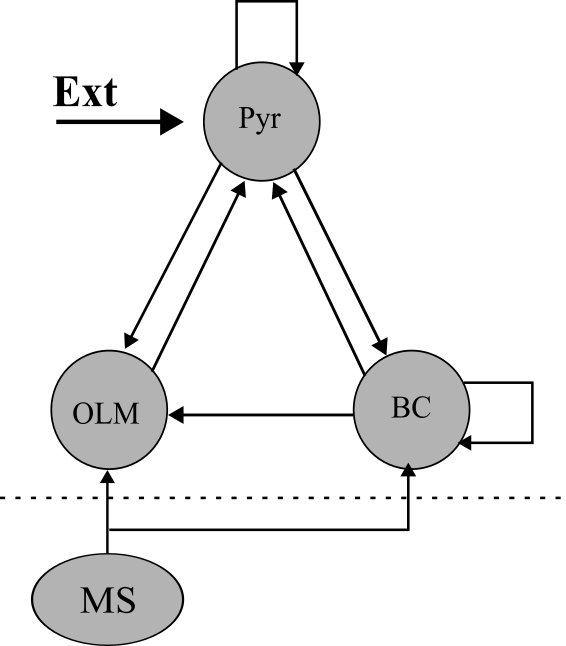
\includegraphics[width=0.5\textwidth]{model_design.png}
    \caption[Schematic of the CA3 network model]{Schematic of the CA3 network model.}
    \begin{minipage}{0.9\textwidth}
        The network comprises of many microcircuits with the connectivity as shown in the above figure. Pyr cells (pyramidal), BC cells (basket cells that inhibit soma),
        OLM cells (oriens lacunosum moleculare interneurons that inhibit dendrites), external inputs (mainly from the entorhinal cortex) to Pyr cells, and MS (medial septum).
        BC and OLM cells are stimulated by Pyr cells, while Pyr cells are inhibited by BC and OLM cells.
        Recurrent connections among Pyr cells are excitatory, whereas those among BC cells are inhibitory.
        OLM cells are inhibited by BC cells. The medial septum (MS) delivers inhibitory inputs every 150 ms to BC and OLM cells.
    \end{minipage}\label{fig:model_design}
\end{figure}\pagebreak

\section{Model implementation: cell parameters}
The model consists of three types of neurons, each with its own set of
parameters and defined cell classes. The parameters for each cell type are
based on the following references:
\begin{enumerate}
    \item \textbf{Basket Cells}: Modeled after \textcite{wangGammaOscillationSynaptic1996},
          featuring standard dynamics for Na and K currents, along with synaptic and leak currents.
          Each cell is modeled as a single compartment and obeys the following current balance equation:
          \begin{equation}
              C_I \frac{dV_I}{dt} = I_{\text{app},I} - I_{\text{Na},I} - I_{\text{K},I} - I_{\text{L},I} - I_{\text{syn},I}
          \end{equation}

          where \(V_I\) is the membrane potential (mV), \(C_I = 1 \, \mu\text{F/cm}^2\)
          is the membrane capacitance, \(I_{\text{app},I}\) is the applied current, and
          \(I_{\text{syn},I}\) is the total synaptic current. The leak current
          \(I_{\text{L},I} = g_{\text{L},I}(V_I - E_{\text{L},I})\) has a conductance
          \(g_{\text{L},I} = 0.1 \, \text{mS/cm}^2\) and reversal potential
          \(E_{\text{L},I} = -65 \, \text{mV}\). All currents are in units of
          \(\mu\text{A/cm}^2\). The sodium \(I_{\text{Na},I}\) and potassium
          \(I_{\text{K},I}\) currents are voltage-dependent spiking currents of the
          Hodgkin-Huxley type.
    \item \textbf{O-LM Cells}: Adapted from \textcite{saragaActiveDendritesSpike2003},
          including additional currents like hyperpolarization-activated (h) and A-type currents.
          Each cell is modeled as a single compartment and obeys the following current balance equation:
          \begin{equation}
              C_O \frac{dV_O}{dt} = I_{\text{app},O} - I_{\text{Na},O} - I_{\text{K},O} - I_{\text{L},O} - I_{\text{h},O} - I_{\text{A},O} - I_{\text{syn},O}
          \end{equation}

          where \(V_O\) is the membrane potential, \(C_O = 1.3 \, \mu\text{F/cm}^2\) is
          the membrane capacitance, \(I_{\text{app},O}\) is the applied current, and
          \(I_{\text{syn},O}\) is the total synaptic current. The leak current
          \(I_{\text{L},O} = g_{\text{L},O}(V_O - E_{\text{L},O})\) with conductance
          \(g_{\text{L},O} = 0.05 \, \text{mS/cm}^2\) and reversal potential
          \(E_{\text{L},O} = -70 \, \text{mV}\). \(I_{\text{Na},O}\), \(I_{\text{K},O}\),
          \(I_{\text{h},O}\), and \(I_{\text{A},O}\) represent the transient sodium,
          delayed rectifier potassium, hyperpolarization-activated (or h) mixed-cation,
          and A-type potassium currents, respectively, all in units of
          \(\mu\text{A/cm}^2\).
    \item \textbf{Pyramidal Cells}: Based on \textcite{miglioreDendriticIhSelectivelyBlocks2004},
          incorporating compartmentalized dynamics for the complex morphology of pyramidal neurons.
          Each cell is modeled as a multi-compartmental neuron with 5 compartments: 1 for basal dendrites (Bdend),
          1 for soma, and 3 for apical dendrites (Adend1, 2 and 3). Each compartment obeys the following current balance equation:
          \begin{equation}
              C_{E_k} \frac{dV_{E_k}}{dt} = I_{\text{app},E_k} - I_{\text{Na},E_k} - I_{\text{K},E_k} - I_{\text{L},E_k} - I_{\text{h},E_k} - I_{\text{A},E_k} - I_{\text{syn},E_k} + I_{\text{conn},E_k}
          \end{equation}

          where \(V_{E_k}\) is the membrane potential of compartment \(k\), \(C_{E_k}\)
          is the membrane capacitance, \(I_{\text{app},E_k}\) is the applied current,
          \(I_{\text{syn},E_k}\) is the total synaptic current, and
          \(I_{\text{conn},E_k}\) represents the current due to electrical coupling
          between compartments. \(I_{\text{L},E_k}\), \(I_{\text{Na},E_k}\),
          \(I_{\text{K},E_k}\), \(I_{\text{h},E_k}\), and \(I_{\text{A},E_k}\) denote the
          leak, transient sodium, delayed rectifier potassium,
          hyperpolarization-activated mixed-cation, and A-type potassium currents for
          compartment \(k\), respectively.
\end{enumerate}

For the full list of cell parameters, see appendix A.\pagebreak

\section{Model implementation: synaptic connections}
The model contained three types of synaptic connections: excitatory, inhibitory
based on AMPA, NMDA and GABA-A receptors. Synapses were modeled by standard
NEURON double-exponential mechanism. The synaptic connections were implemented
as follows:

\begin{table}[htbp]
    \centering
    \caption[Synaptic Parameters for the Connectivity Between Neurons in the Model]{Synaptic Parameters for the Connectivity Between Neurons in the Model: Pre- and postsynaptic receptor types are given for each cell type.
        The time constants \(\tau_1\) and \(\tau_2\) are in milliseconds.
        \(\tau_1\) is the rise time constant, the time it takes for synaptic conductance to increase from baseline to peak.
        \(\tau_2\) is the decay time constant, the time it takes for the conductance to decrease from peak to baseline.
        The conductance indicates the strength of the synaptic connection and its ability to conduct ionic current across the postsynaptic membrane.
        This influences the extent to which the synaptic input can depolarize the postsynaptic neuron and is in nanoSiemens (nS).}
    \begin{tabular}{lllccc}
        \hline
        Presynaptic & Postsynaptic & Receptor & \(\tau_1\) (ms) & \(\tau_2\) (ms) & Conductance (nS) \\
        \hline
        Pyramidal   & Pyramidal    & AMPA     & 0.05            & 5.3             & 0.02             \\
        Pyramidal   & Pyramidal    & NMDA     & 15              & 150             & 0.004            \\
        Pyramidal   & Basket       & AMPA     & 0.05            & 5.3             & 0.36             \\
        Pyramidal   & Basket       & NMDA     & 15              & 150             & 1.38             \\
        Pyramidal   & OLM          & AMPA     & 0.05            & 5.3             & 0.36             \\
        Pyramidal   & OLM          & NMDA     & 15              & 150             & 0.72             \\
        Basket      & Pyramidal    & GABA-A   & 0.07            & 9.1             & 0.72             \\
        Basket      & Basket       & GABA-A   & 0.07            & 9.1             & 4.5              \\
        Basket      & OLM          & GABA-A   & 0.07            & 9.1             & 0.0288           \\
        OLM         & Pyramidal    & GABA-A   & 0.2             & 20              & 72               \\
        MS          & Basket       & GABA-A   & 20              & 40              & 1.6              \\
        MS          & OLM          & GABA-A   & 20              & 40              & 1.6              \\
        \hline
    \end{tabular}\label{tab:synaptic_parameters}
\end{table}

\section{Model implementation: stimulation and noise}
The model was activated by external inputs originating from the entorhinal
cortex, which were then transmitted to the pyramidal cells. Background random
excitatory and inhibitory inputs were received by the OLM, basket cells, and
the soma of the pyramidal cells via their AMPA, NMDA, and GABA-A receptors as
shown in table~\ref{tab:synaptic_parameters}. The mechanism by which noise was
applied to the model was defined via NEURON simulator's \textit{NetStim}
object. This object type generated spike train according to a set of parameters
such as stimulus interval, noise variability (Poisson-like), weight, target,
start and delay times. These parameters can bee viewed in Appendix A.

Similarly, the distal dendritic compartments of the pyramidal cells also
received comparable inputs through the same types of receptors. Connections
such as OLM to pyramidal cell, basket to pyramidal cell, basket-basket
recurrent connections, and medial septum to OLM and basket cell connections
were mediated through GABA-A receptors. Additionally, the medial septum
provided inhibitory inputs to the basket and OLM cells at intervals of 150 ms.

\section{Simulations}
For the simulations, the model was implemented in NEURON version 7.6.3. The
simulations were run on a Linux GNOME (v22.04) desktop computer with 2 Xeon CPU
E5--2699 v3 CPUs with 32 physical cores @ 2.3GHz for multi-threading, a Nvidia
GTX 4060 graphics card, and 256 GB of RAM\@. Trials were run for 5000 ms with a
time integration step of 0.1 ms resulting in 50.000 simulation steps per trial
dataset. Random seeds were used to generate the external noise, connections and
cells for each trial and remained constant between trials and between
experiments. The number of trials varies between experiments and are specified
in their respective sub-sections that follow. In the network, the individual
cells were assigned a global identifier to which all the data was associated in
the same ascending order for each trial. The first 800 cells were always
pyramidal cells, the next 200 were basket cells and the last 200 were OLM
cells. For each trial, the individual cell spike times were saved for the
entire duration of the simulation. Pyramidal cell membrane soma voltage data
was saved per cell in order to calculate the LFP signal (necessary for
theta-gamma calculations).

\subsection{Baseline activity}
In order to obtain baseline activity in the network as shown in figure
~\ref{fig:model_design}, current injections were added (\textbf{Pyramidal
    cells:} 50 pA\@; \textbf{OLM cells:} -25 pA). At Baseline, the network
generates theta-modulated gamma oscillations activity. This activity was
measured from the Local Field potential (LFP) in the network. The LFP was
simulated by a sum difference between membrane potential of the distal apical
and basal dendritic compartment over all pyramidal cells. As discussed in the
cell parameters section, all cells contained leak current, transient sodium
current \(I_{\text{Na}}\), and delayed rectifier current \(I_{K, \text{-}
        \text{dr}}\) to allow for action potential generation. On average, the firing
rates were \(2.36 \pm 0.024\) Hz for pyramidal cells, \(16.05 \pm 0.15\) Hz for
basket cells and \(0.96 \pm 0.027\) Hz for O-LM interneurons at baseline in the
original \parencite{sanjayImpairedDendriticInhibition2015}. However, it should
be noted that our custom implementation of the same model had a slightly
lowered baseline (see the results section). The reason for this discrepancy is
unknown and is a potential source of error in the results. 50 trials total were
done for the baseline activity and averaged.

\subsection{Model validation}
In order to test the implementation of the model, results from the article were
replicated, namely figures 6A, B and C from
\textcite{sanjayImpairedDendriticInhibition2015}. In this replicated experiment
the OLM to pyramidal cells connection weight was reduced in decrements of 0.1x
times the baseline from 1.0 to 0.0. In addition to reduced connection strength,
the external noise fed into the pyramidal cells was increased in increments of
0.1X times the baseline from 1.0 to 2.0. By reducing the connectivity from OLM
to pyramidal cells, dendritic inhibition was impaired and potential
epileptiform activity was induced. The original results on which the validation
experiment focussed on, were the following three aspects: changes in firing
rates per population, the changes in dominant theta and gamma frequencies, and
finally the changes in the power of the theta and gamma oscillations.

\subsection{Sodium and potassium variants}
In this experiment, the sodium and potassium conductances of the all cell types
cells were changed from 0.5x to 1.5x times the baseline in increments of 0.1.
The changes were induced in separate experiments for each of the three cell
types, so 6 experiments in total were conducted: 3 for sodium and 3 for
potassium. These induced changes were done in order to investigate the effect
of the conductances on the network activity and the influence of individual
cell types on the same metrics as in the model validation experiment. 20 trials
each were done per condition (6 total conditions) and the results were
averaged.

\subsection{External noise variants}
In this experiment, the external noise fed into the pyramidal cells was set a
new baseline for the 1.0x condition, which was 20 times that of the original
\textcite{sanjayImpairedDendriticInhibition2015} model. Reduced OLM to pyr
connections were kept at 10\% of the original baseline. This was done because
in the original article, epileptic activity was induced by feeding in 20 times
more external noise at reduced dendritic inhibition. This condition was tested
as a special condition in figure 7 of the article, and was expanded upon
because of the occurrence of a depolarization block in the basket cell spike
activity. This depolarization block occurrence was assumed to be the epileptic
state in which the network is found at such conditions. This new baseline was
changed times a range of pyramidal noise factors of the following values: 0.65,
0.70, 0.75, 0.80, 0.85, 0.90, 0.95, 1.00, 1.10, 1.20, and 1.30. In addition to
the range of noise factors, pyramidal conductances \(g_{\text{Na}}\) and
\(g_{\text{K}}\) were modified over a range of 0.5x to 1.5x times the baseline
in increments of 0.1. 15 trials were done per noise condition and the results
were averaged.

\subsection{Recurrent connection strength variants}
In this experiment, the recurrent connection strength between basket cells was
modified over the following range: 1.00, 1.05, 1.10, 1.15 and 1.20 times the
baseline. This was done in order to investigate the possibility of rescuing the
epileptic network back to baseline activity by increasing the strength of soma
inhibition. Similarly to the external noise variants, \(g_{\text{Na}}\) and
\(g_{\text{K}}\) were modified over a slightly tighter range of plus or minus
25\% of the baseline and including baseline of 1.00. Again, the OLM to
pyramidal connection weight was kept at 10\% in order to be able to evoke the
depolarization block in basket cell spike activity, while also feeding the 20x
external noise to the pyramidal cells. 15 trials were done per condition and
the results were averaged.

\subsubsection{Detection of epileptiform activity (Experiment: External noise variants)}
The detection of epileptic activity depends on the spiking activity of the
basket cells, which according to results of figure 7 from the
\textcite{sanjayImpairedDendriticInhibition2015} article occurs in the presence
of great external drive from the pyramidal cells of at least 20 times the
baseline and with reduced dendritic inhibition by the OLM cells. Detection of a
depolarization block in the basket cells was done by calculating the convoluted
fire rates of the basket cell population.

\noindent The systematic approach to analyzing basket cell firing rates through
convolution with a Gaussian window was as follows:
\begin{itemize}
    \item \textbf{Extracting Spike Times:} The \lstinline{get_spike_times_for_basket_cells}
          function is used for iterating over a range of GIDs. This process collects spike times from
          all basket cells and concatenates them, constructing a continuous signal of neural activity.

    \item \textbf{Creating Time Series:} Spike times are converted into a binary series
          using \lstinline{create_time_series}. Each neural firing event is denoted by a '1' in a
          zero-initialized array at the corresponding time index.

    \item \textbf{Applying Gaussian Convolution:} The \lstinline{apply_gaussian_convolution}\newline
          function smooths the time series. It convolves the series with a Gaussian window, normalized
          to sum to one, yielding a signal that mirrors the firing rates over time.

    \item \textbf{Summing Convolved Signals:} Collective firing behavior is analyzed by
          \lstinline{get_convolved_signal_per_neuron}. It applies Gaussian convolution to individual
          neuron time series and sums them, forming an aggregated firing rate signal.

    \item \textbf{Detecting Depolarization Blocks:} The \lstinline{detect_depolarization_blocks}
          function identifies reduced activity periods by analyzing the convolved signal for intervals
          that remain below a set threshold for a specified minimum duration.
\end{itemize}

\noindent For detecting depolarization blocks in the basket cell population, the
methodology was as follows:
\begin{itemize}
    \item Establishing a signal threshold indicating a depolarization block.
    \item Excluding initial transient analysis to prevent false positives.
    \item Identifying threshold crossings that mark the start and end of depolarization
          blocks.
    \item Applying a minimum duration filter to these blocks.
    \item Summarizing and reporting the total duration of all valid depolarization blocks
          in the trial.
\end{itemize}

\noindent A check was performed if the convoluted signal remained beneath a fixed
threshold of 0.001 for at least 100 ms. This threshold was defined non-zero,
yet tiny as in the depolarization block there are no firing neurons in the
basket population. The first 50 ms of the signal were excluded to avoid false
positives. If the signal remained beneath the threshold for at least 100 ms,
the condition was considered to be in a depolarization block state. This was
done for each trial individually.\pagebreak

\subsubsection{Detection of epileptiform activity (Experiment: Recurrent connection strength variants)}

\subsubsection{Burst detection around depolarization block onset}